\documentclass{./../div_teaching_slides}
\usepackage{setspace}

\begin{document}
\title{ECON 340 \\ Economic Research Methods}
\author{Div Bhagia}
\date{Lecture 9: Distribution, Expectation, and Variance}

\begin{frame}[noframenumbering, plain]
\maketitle
\end{frame}

%%%%%%%%%%%% 
\begin{frame}{Taking stock}
We have learned how to describe variables in the data using: \\ \vspace{0.5em}

\begin{witemize}
\item Empirical distribution 
\item Mean and median
\item Variance and standard deviation
\item Correlation and covariance
\end{witemize}
\end{frame}

%%%%%%%%%%%% 
\begin{frame}{Random Sampling}
\begin{witemize}
\item Often, data is available only for a sample of the population
\item Ideally, we want a sample \textit{representative} of the population we are interested in and not a \textit{biased} sample
\item We can achieve this by taking a \textit{random sample} from the population 
\item Random sample: each unit from the population has an equal probability of being chosen
\end{witemize}
\end{frame}

%%%%%%%%%%%% 
%\begin{frame}{Simple Example}
%\vspace{-0.25em}
%\textit{Say, we want to take a random sample of 2 from a population of 5.} \\ \vspace{0.5em}
%\begin{columns}[T]
%\begin{column}{0.3\textwidth}
%\textit{Population}: \\
%\( X_1 = \$60,000 \) \\
%\(X_2 = \$40,000 \) \\
%\( X_3 = \$40,000 \) \\
%\(X_4 = \$50,000 \) \\
%\(X_5 = \$60,000 \) \\~\\
%\textit{Population mean}:
%\(\mu = \$50,000\)
%\end{column}	
%\begin{column}{0.625\textwidth}
%Pick a sample randomly: \href{https://tools-unite.com/tools/random-picker-wheel?inputs=1:1,2:1,3:1,4:1,5:1}{\blue{Spin a Wheel}} \\ \vspace{0.5em}
%\textit{Attempt 1}  \\ \vspace{0.25em}
%$ \bar{X}_1 =  $ \\~\\
%\textit{Attempt 2}  \\ \vspace{0.25em}
%$ \bar{X}_2 =  $ \\~\\
%\textit{Attempt 3}  \\ \vspace{0.25em}
%$ \bar{X}_3 = $
%\end{column}	
%\end{columns}
%\end{frame}

%%%%%%%%%%%%%%%%%%%%
\begin{frame}{Simple Example}
\begin{witemize}
\item We are interested in the average GPA of students in our population of interest
 \item Say our population has 10 students and we take a random sample of 5
\item Interactive example: \href{https://dbhagia.shinyapps.io/randomsample/}{dbhagia.shinyapps.io/randomsample}
\end{witemize}
\end{frame}


%%%%%%%%%%%% 
\begin{frame}{Random Sampling}
\begin{witemize}
\item We can get different values of the sample mean depending on the sample we pick
\item Sample mean is a \textit{random variable}!
\item Then what can we infer about the population mean from the sample mean?
\item But before that, what is a random variable?
\end{witemize}
\end{frame}


%%%%%%%%%%%% 
\begin{frame}{Random Variables}
\begin{witemize}
  \item \textit{Random variable} is a numerical summary of a random outcome. 
  \item Examples:  outcome from a coin toss or a die roll, or number of times your wireless network fails before a deadline, etc.
  \item Random variables can be \textit{discrete} or \textit{continuous}
  \item Discrete random variables take a discrete set of values, like $0, 1, 2,...$
  \item Continuous random variables take on a continuum of possible values
\end{witemize}
\end{frame}

%%%%%%%%%%%%
\begin{frame}{Discrete Random Variables}
\begin{witemize}
  \item \textit{Probability distribution} of a discrete random variable: all possible values of the variable and their probabilities. 
$$ f(x) = Pr(X=x) $$
where $0 \leq f(x) \leq 1$ for all $x$ and $\sum_x f(x) = 1$.

\vspace{1em}
\item \textit{Cumulative probability distribution} gives the probability that the random variable is less than or equal to a particular value.
$$ F(x) = Pr(X \leq x) = \sum_{x' \leq x} f(x') $$ \\
\end{witemize}
\end{frame}

%%%%%%%%%%%%
\begin{frame}{Discrete Random Variable: Example}
$X$: outcome from rolling a die	\\
\begin{center}
	\begin{tabular}{ccc}
$X$ & $f(X)$ & $F(X)$ \\
\hline
$1$ & $1/6$ & $1/6$\\
$2$ & $1/6$ & $2/6$ \\
$3$ & $1/6$ & $3/6$ \\
$4$ & $1/6$ & $4/6$ \\
$5$ & $1/6$ & $5/6$ \\
$6$ & $1/6$ & $1$\\
\end{tabular}
\end{center}
\vspace{0.5em}

Also referred to as probability distribution function (PDF) and cumulative distribution function (CDF).
\end{frame}

%%%%%%%%%%%%
%\begin{frame}{Bernoulli Random Variable}
%\textit{Bernoulli Random Variable.} A special type of discrete random variable that only takes two values 1 and 0. It is also called a \textit{binary} variable. 
%
%$$ X = \begin{cases} 
% 	1 \quad \text{with probability $p$} \\
% 	0 \quad \text{with probability $1-p$} 
% \end{cases}
%$$
%\end{frame}

%%%%%%%%%%%%
\begin{frame}{Continuous Random Variable}
\begin{witemize}
\item For continuous random variables, due to a continuum of possible values, it is not feasible to list the probability of each possible value.
\item So instead, the area under the \textit{probability density function} $f(x)$ between any two points gives the probability that the random variable falls between those two points.
\item \textit{Cumulative probability distribution} for continuous RVs is defined as before $F(x) = Pr(X \leq x)$.
\end{witemize}
\end{frame}


%%%%%%%%%%%%
\begin{frame}{Probability Density Function}
\vspace{1.5em}
\centering
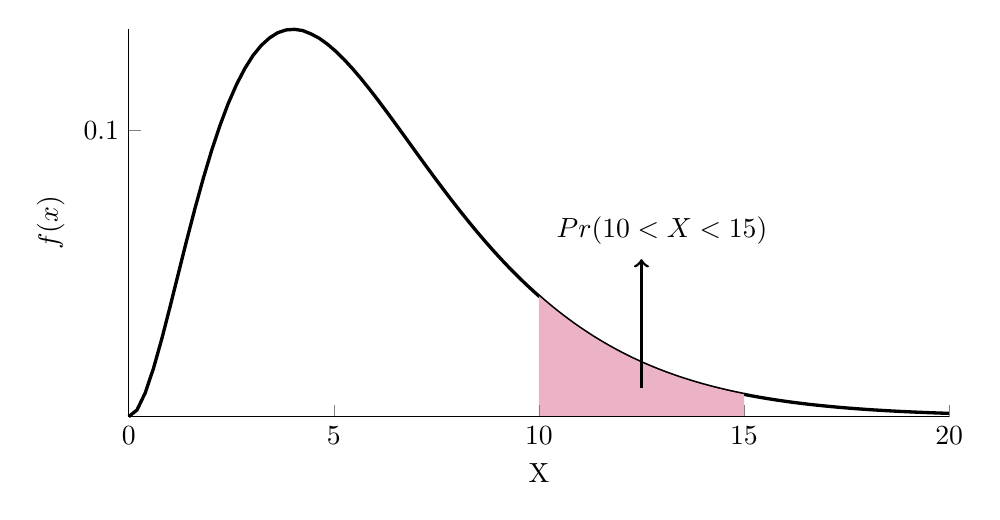
\begin{tikzpicture}[
    declare function={gamma(\z)=
    2.506628274631*sqrt(1/\z)+ 0.20888568*(1/\z)^(1.5)+ 0.00870357*(1/\z)^(2.5)- (174.2106599*(1/\z)^(3.5))/25920- (715.6423511*(1/\z)^(4.5))/1244160)*exp((-ln(1/\z)-1)*\z;},
    declare function={gammapdf(\x,\k,\theta) = 1/(\theta^\k)*1/(gamma(\k))*\x^(\k-1)*exp(-\x/\theta);}
]
\begin{axis}[
  no markers, domain=0:20, samples=100,
  axis lines*=left, xlabel=X, ylabel=$f(x)$,
  %every axis y label/.style={at=(current axis.above origin),anchor=south},
  height=6.5cm, width=12cm,
  xtick={0,5,10,15,20}, ytick={0.1},
  enlargelimits=false, clip=false, axis on top,
  ]
\addplot [very thick,black] {gammapdf(x,3,2)};
\addplot [fill=purple!30, draw=none, domain=10:15] {gammapdf(x,3,2)} \closedcycle;;
\draw[->, line width=1pt](axis cs: 12.5, 0.01)--(axis cs: 12.5, 0.055);
\node at (axis cs: 13, 0.065) {$Pr(10 <X<15)$};
\end{axis}
\end{tikzpicture}
\end{frame}


%%%%%%%%%%%%
\begin{frame}{How to calculate the area under the curve?}
\begin{witemize}
  \item Area under the curve is calculated using an \textit{integral} (just like a sum but for continuous variables)
  \item However, don't sweat, in most cases a statistical program or old-school tables (in the back of textbooks) can help us find these areas for commonly used distributions
  \item We will now define expectation and variance for the discrete case, but it is generalizable to continuous RVs
\end{witemize}
\end{frame}


%%%%%%%%%%%%
\begin{frame}{Expectation}
\begin{witemize}
  \item \textit{Expectation}: average value of the random variable over many repeated trials or occurrences
  \item Computed as a weighted average of the possible outcomes, where the weights are the probabilities
  \item The expectation of $X$ is also called the \textit{expected value} or the \textit{mean} and is denoted by $\mu_X$ or $E(X)$
  $$ \mu_X = E(X) = \sum_x f(x) x $$
  \end{witemize}
\end{frame}

%%%%%%%%%%%%%%%%%%%%
\begin{frame}{Example}
\vskip-0.5em
An outdoor market vendor sells handmade crafts.
\begin{center}
\begin{tabular}{|l|c|c|}
\hline
\textbf{Weather} & \textbf{Probability} & \textbf{ Sales (\$)} \\ \hline
No rain                    & 0.6                 & 300                        \\ \hline
Light rain                 & 0.3                 & 150                        \\ \hline
Heavy rain                 & 0.1                 & 50                         \\ \hline
\end{tabular} 
\end{center} \vskip0.75em
$$ E(Sales) = (0.6 \times 300) + (0.3 \times 150) + (0.1 \times 50) = \$230  $$\vskip0.75em
\pause \textit{Daily sales will fluctuate due to randomness of the weather. However, if this day were to repeat itself multiple times, the vendor would, on average, expect to achieve daily sales of \$230.}
\end{frame}


%%%%%%%%%%%%%
%\begin{frame}{Roll of a Die}
%The expected value from the roll of a die
%$$ E(X) = \frac{1}{6} \cdot 1 +  \frac{1}{6} \cdot 2 +  \frac{1}{6} \cdot 3 +  \frac{1}{6} \cdot 4 +  \frac{1}{6} \cdot 5 +  \frac{1}{6} \cdot 6 =\frac{21}{6} = 3.5 $$
%\end{frame}

%%%%%%%%%%%%
\begin{frame}{Variance and Standard Deviation}
The variance and standard deviation measure the dispersion or the ``spread''. \\
$$ \sigma^2_X =   Var(X) = E[(X-\mu_X)^2] =  \sum_{x} (x-\mu_X)^2 f(x) $$ \\
Variance is the expected value of the squared deviation of $X$ from its mean. \\~\\
\textit{In our example, the variance will capture the potential variability or fluctuation in sales on any given day compared to the average (expected value).}
\end{frame}

%%%%%%%%%%%%%%%%%%%%
\begin{frame}{Example}
\vskip-0.5em
An outdoor market vendor sells handmade crafts. \\ \vskip1.25em
\begin{center}
\begin{tabular}{|l|c|c|}
\hline
\textbf{Weather} & \textbf{Probability} & \textbf{ Sales (\$)} \\ \hline
No rain                    & 0.6                 & 300                        \\ \hline
Light rain                 & 0.3                & 150                        \\ \hline
Heavy rain                 & 0.1                & 50                         \\ \hline
\end{tabular} 
\end{center} \vskip0.5em
\begin{align*}
E(Sales) &= \red{0.6} \cdot (300) + \red{0.3} \cdot (150) + \red{0.1} \cdot (50) = \$230 \\~\\
Var(Sales) &= \red{0.6} \cdot (300 - 230)^2 + \red{0.3} \cdot (150 - 230)^2 + \red{0.1} \cdot (50 - 230)^2 \\
&= 8100
\end{align*}
\end{frame}

%%%%%%%%%%%%%
%\begin{frame}{Roll of a Die}
%Expected value 
%$$ E(X) = \frac{1}{6} \cdot 1 +  \frac{1}{6} \cdot 2 +  \frac{1}{6} \cdot 3 +  \frac{1}{6} \cdot 4 +  \frac{1}{6} \cdot 5 +  \frac{1}{6} \cdot 6 =\frac{21}{6} = 3.5 $$
%\vspace{1em}
%
%Variance
%$$ Var(X) = (-2.5)^2.\frac{1}{6} + (-1.5)^2.\frac{1}{6} + (-0.5)^2.\frac{1}{6} + (0.5)^2.\frac{1}{6}  $$
%$$ \quad \quad + (1.5)^2.\frac{1}{6}   + (2.5)^2.\frac{1}{6} = \frac{17.5}{6} $$ 
%\end{frame}

%%%%%%%%%%%%
\begin{frame}{Variance and Standard Deviation}
Alternative formula for the variance:  $$Var(X) = E[(X-\mu_X)^2] = E(X^2)-\mu_X^2$$ \\~\\
Since variance is in units of the square of $X$, therefore we use \textit{standard deviation} which is the square-root of variance
$$ \sigma_X = \sqrt{\sigma^2_X}  $$

\textit{For our example, standard deviation of sales is $\sqrt{8100} = \$ 90 $. 
}\end{frame}

%%%%%%%%%%%%
\begin{frame}{Transformations of Random Variables}
 If you shift every outcome by some constant  $a$, \\~\\
  \begin{witemize}
  \item Mean also shifts by $a$:
  $$E(X + a) = E(X) + a $$
  \item Variance is unchanged: 
   $$ Var(X + a) = Var(X) $$
  \end{witemize}
\end{frame}

%%%%%%%%%%%%%%%%%%%%
\begin{frame}{Shifting the Distribution}
\vfill
\centering
\begin{tikzpicture}
\begin{axis}[
    no markers, 
    %domain=-2:15, 
    samples=100,
    ymin=0,
    axis lines*=left, 
    xlabel=,
    ylabel=$f(x)$,
    height=7cm, 
    width=16cm,
    xtick=\empty, 
    ytick=\empty,
    clip=false,
    axis on top,
    grid = major,
    hide y axis
    ]
% Distributions
\addplot [black, very thick, domain=-3:11] {gauss(4,2)};
\addplot [purple, very thick, domain=2:16] {gauss(9,2)};
% Means
\draw [color=black, very thick, dashed] (axis cs:4,0) -- (axis cs:4,0.2);
\node[below] at (axis cs:4, 0) {$\mu_X$};
\draw [color=purple, very thick, dashed] (axis cs:9,0) -- (axis cs:9,0.2);
\node[below] at (axis cs:9, 0) {$\purple{\mu_X + a}$};
% Random point
\draw [color=black, very thick, dashed] (axis cs:1.5,0) -- (axis cs:1.5,0.09);
\node[below] at (axis cs:1.5, 0) {$x$};
\draw [color=purple, very thick, dashed] (axis cs:6.5,0) -- (axis cs:6.5,0.09);
\node[below] at (axis cs:6.5, 0) {$\purple{x + a}$};
% Distance from the mean
\draw [color=black, thick, <->] (axis cs:1.5,0.05) -- (axis cs:4,0.05) node [midway, above] {$\sigma_X$};
\draw [color=black, thick, <->] (axis cs:6.5,0.05) -- (axis cs:9,0.05) node [midway, above] {$\sigma_X$};
\end{axis}
\end{tikzpicture}
\end{frame}


%%%%%%%%%%%%
\begin{frame}{Transformations of Random Variables}
 If you scale every outcome by some constant $b$, \\~\\
  \begin{witemize}
  \item Mean is also scaled by $b$:
  $$E(bX) = bE(X) $$
  \item Variance is scaled by $b^2$:
   $$ Var(bX) = b^2 Var(X) $$
  \end{witemize}
\end{frame}

%%%%%%%%%%%%%%%%%%%%
\begin{frame}{Scaling the Distribution}
\vfill
\centering
\begin{tikzpicture}
\begin{axis}[
    no markers, 
    %domain=-2:15, 
    samples=100,
    ymin=0,
    axis lines*=left, 
    xlabel=,
    ylabel=$f(x)$,
    height=7cm, 
    width=16cm,
    xtick=\empty, 
    ytick=\empty,
    clip=false,
    axis on top,
    grid = major,
    hide y axis
    ]
% Distributions
\addplot [black, very thick, domain=0:8] {gauss(4,1)};
\addplot [purple, very thick, domain=2:12] {gauss(7,2)};
% Means
\draw [color=black, very thick, dashed] (axis cs:4,0) -- (axis cs:4,0.4);
\node[below] at (axis cs:4, 0) {$\mu_X$};
\draw [color=purple, very thick, dashed] (axis cs:8,0) -- (axis cs:8,0.175);
\node[below] at (axis cs:8, 0) {$\purple{b\mu_X}$};
% Random point
\draw [color=black, very thick, dashed] (axis cs:3,0) -- (axis cs:3,0.23);
\node[below] at (axis cs:3, 0) {$x$};
\draw [color=purple, very thick, dashed] (axis cs:6,0) -- (axis cs:6,0.175);
\node[below] at (axis cs:6, 0) {$\purple{bx}$};
% Distance from the mean
\draw [color=black, thick, <->] (axis cs:3,0.15) -- (axis cs:4,0.15) node [midway, above] {$\sigma_X$};
\draw [color=black, thick, <->] (axis cs:6,0.1) -- (axis cs:8,0.1) node [midway, above] {$b\sigma_X$};
\end{axis}
\end{tikzpicture}
\end{frame}


%%%%%%%%%%%%
\begin{frame}{Transformations of Random Variables}
More generally, if $X$ is a random variable and $$Y=a+bX$$
Then $Y$ is also a random variable with 
$$ E(Y) = a + b E(X) \quad \quad Var(Y) = b^2 Var(X) $$ \\
In addition, a linear transformation of a random variable does not change the shape of the distribution. 
\end{frame}

%%%%%%%%%%%%
%\begin{frame}{Example}
%Flip a coin to gain \$10 or loose \$10. 
%\begin{center}
%\renewcommand*{\arraystretch}{1.25}
%\begin{tabularx}{0.9\textwidth}{rcccc}
%$x$ & $f(x)$ & $xf(x)$ & $(x-E(X))^2$ & $f(x)(x-E(X))^2$\\
%\hline
%10 & 0.5 & 5 & (10)$^2$ & 50 \\
%-10 & 0.5 & -5 & (-10)$^2$ & 50  \\
%\hline
%& & 0 & & 100 \\
%\hline
%\end{tabularx}
%\end{center}
%So we have that $E(X) = 0$ and $var(X)=100$. \\~\\
%Now say, $Y = X-5$ and $Z=0.5X$. What is the expectation and variance of $Y$ and $Z$?
%\end{frame}

\begin{frame}{Example}
\vskip-0.75em
The market vendor offered you a job, you get \$20 and 10\% commission ($Y$) on sales ($X$) per day.
$$ Y = 20 + 0.1 X $$ \\ \vskip0.15em
\begin{center}
\begin{tabular}{|l|c|c|c|}
\hline
\textbf{Weather} & \textbf{Probability} & \textbf{ X} & \textbf{Y} \\ \hline
No rain                    & 0.6                 & 300   &  20 + 0.1(300) = 50                     \\ \hline
Light rain                 & 0.3                 & 150   & 20 + 0.1(150) = 35                    \\ \hline
Heavy rain                 & 0.1                 & 50    &  20 + 0.1(50) = 25                   \\ \hline
\end{tabular} 
\end{center} 
\begin{align*}
E(Y) &=  20 + 0.1 E(X) = 20 + 0.1(230) = 43 \\
Var(Y) &= 0.1^2 \cdot Var(X) = 0.01 (8100) = 81 \\
SD(Y) &= \sqrt{81} = 9 \ (= 0.1 SD(X))
\end{align*}
\end{frame}

%%%%%%%%%%%%
\begin{frame}{Standardized Random Variables}
A random variable can be transformed into a random variable with mean 0 and variance 1 by subtracting its mean and then dividing by its standard deviation, a process called standardization. \\~\\
$$ Z = \frac{X-\mu_X}{\sigma_X} $$ \\~\\
Here, $E(Z) = 0$ and $\sigma_Z = 1$.
\end{frame}

%%%%%%%%%%%%%%%%%%%%
\begin{frame}{Coming Up}
\begin{witemize}
  \item Problem Set 2 is due by the end of the day today
\item Research Paper Submission I due next week on Tuesday
\end{witemize}

  
\end{frame}

\end{document}